\section{Das Speichermodell von Java}\label{sec:memory-model}

Es soll nun ein Beispiel betrachtet werden, um das Speicherproblem näher zu erläutern, das Value Types lösen sollen.
Es sollen einige ganzzahlige Punkte im zweidimensionalen Raum gespeichert werden, die einen Pfad bilden.
Die Punkte sind als Objekte mit zwei \code{int}-Feldern modelliert, der Pfad als Array von Punkten.
Bei einer Pfadlänge von drei berechnet sich der Speicherverbrauch wie folgt:

\begin{equation}
    \SI{24}{\Byte} + 3 \cdot \SI{8}{\Byte} + 3 \cdot (\SI{16}{\Byte} + 2 \cdot \SI{4}{\Byte}) = \SI{120}{\Byte}\label{eq:memory-usage-current}
\end{equation}

Die Größe eines Array-Headers beträgt $\SI{24}{\Byte}$~\cite{compressed-oops}.
Ein Objekt, das zwei \code{int}-Werte beeinhaltet, benötigt auf einer 64-bit \ac{jvm} $\SI{8}{\Byte}$ für die Referenz selber, $\SI{16}{\Byte}$\footnote{Mit dem \ac{jvm}-Flag \code{-XX:+UseCompressedOops} könnte dies auf $\SI{12}{\Byte}$ reduziert werden, allerdings kommen dann $\SI{4}{\Byte}$ Padding hinzu, da die Größe von Objekten im Heap ein Vielfaches von $\SI{8}{\Byte}$ sein muss~\cite{compressed-oops}.} für den Objekt-Header und je $\SI{4}{\Byte}$ für die beiden \code{int}-Werte~\cite{compressed-oops}.
Mit drei Objekten ergibt sich also insgesamt ein Speicherverbrauch von $\SI{120}{\Byte}$.

Das gleiche Beispiel soll nun mit Value Types realisiert werden.
Dabei entfallen die Objekt-Header und Referenzen vollständig.
Der neue Speicherverbrauch berechnet sich also wie folgt:

\begin{equation}
    \SI{24}{\Byte} + 3 \cdot 2 \cdot \SI{4}{\Byte} = \SI{48}{\Byte}\label{eq:memory-usage-inline}
\end{equation}

Folglich konnten $\SI{72}{\Byte}$ eingespart werden.
Der Effekt wird verstärkt, wenn das Array mehr Elemente enthält.
Zu beachten ist auch, dass die gesamten Daten des Arrays mit einer Größe von $\SI{48}{\Byte}$ in eine Cache-Zeile passen, wenn bei deren Größe von $\SI{64}{\Byte}$ ausgangen wird.

In Abbildung~\ref{fig:memory-usage} erfolgt eine grafische Darstellung des verringerten Speicherverbrauchs.
Sie zeigt links das Speicherlayout in heutigen \acp{jvm} und rechts das Speicherlayout, wenn Value Types für die Punkte verwendet werden.

\begin{figure}[htp]
    \centering
    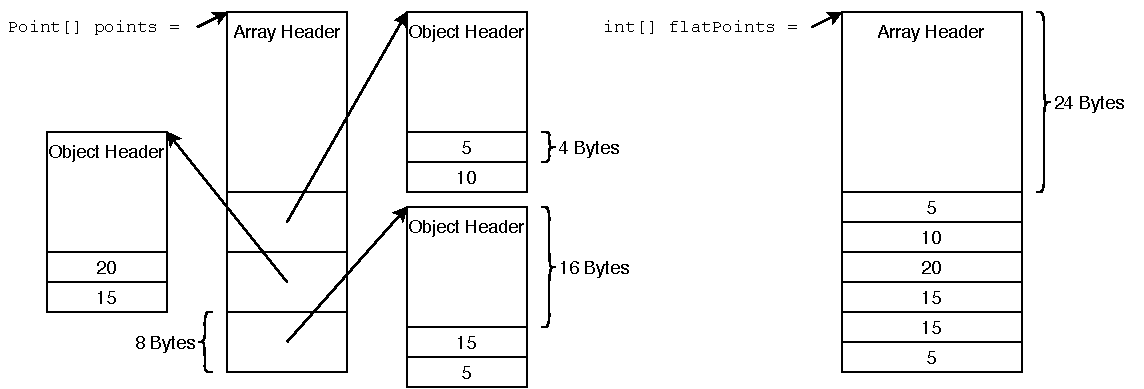
\includegraphics[width=\textwidth]{img/memory-usage.pdf}
    \vspace{-3ex}
    \caption{Vergleich des Speicherlayouts eines Arrays von Punkten heute (links) und mit Value Types (rechts)}
    \label{fig:memory-usage}
\end{figure}

Neben Punkten lassen sich mit Value Types eine Vielzahl von neuen Datentypen definieren, die breite Anwendung finden können.
Dazu gehören im Bereich der numerischen Datenverarbeitung komplexe, vorzeichenlose und Dezimalzahlen, Binärzahlen größer als 64 bit und Vektoren, die auf modernen \acp{cpu} effizient verarbeitet werden können.
Auch algebraische Datentypen wie \code{Optional}, \code{Either}, \code{Unit} und Tupel sind wichtige Einsatzmöglichkeiten.
Letztere benötigen jedoch besondere Sprachunterstützung, die noch nicht Teil des Projekts ist.
